\documentclass[11pt]{article}
\usepackage[margin=1in]{geometry}
\usepackage{booktabs,graphicx,amsmath}
\title{An FSDS weight on the Q-index\\
\large Same table, a penalty on the action the stale policy would take}
\author{}
\date{}
\begin{document}
\maketitle

\section{Where the weight sits}

The control task already has a visit-bonus table \(Q(s,a)\). The state \(s\) is
the three-way sign of two known reference scores and the step. Putting the
pseudo-outcome share into that state split the visits and raised the excess
on the sign flip. The weight below does not add a coordinate.

Four reference policies are scored on every batch, on the same calendar as
the scorecard race. The weight uses the two directional scores, the same two
whose signs form the state. Write \(w_{(1)}\) and \(w_{(2)}\) for the larger
and the smaller of their shares, and \(a_{(1)}(s)\), \(a_{(2)}(s)\) for the
actions they prescribe. The penalty on an action is the share gap, and only
on the action of the higher share, and only in states where the two actions
differ:
\[
\delta(s,a)=(w_{(1)}-w_{(2)})\,1\{a=a_{(1)}(s)\}\,1\{a_{(1)}(s)\neq a_{(2)}(s)\}.
\]
The decision index is
\[
Q(s,a)+c(s,a)-\eta\sigma\cdot\frac{H-h}{H}\cdot\delta(s,a),
\]
with \(\eta\in\{1,2\}\) and \(\sigma\) the scale of the four reference
returns on the first six rounds. The factor \((H-h)/H\) charges the
episode-level penalty once along the horizon. Equal shares give
\(\delta=0\), so the weight is inert while the two scores still carry the
same residual. Agreement of the two actions also gives \(\delta=0\): the
weight does not tax a button both scores would press.

The backup is unchanged. The target is the observed reward plus the max of
the next raw table. The share is a statement about which reference score
still explains the outcome. It is not a reward, so it does not enter the
value being learned. An unvisited cell still carries the large visit bonus,
so the weight cannot hide an action the table has not tried.

One variant turns the weight off on a round whose largest share belongs to
the zero policy. That is the sign-flip symptom: the null score holds the
mass, and a penalty aimed at a stale action has nothing stale to point at.
Across pools, the fraction of post-shift rounds in which the zero policy
holds the share has median 0.00 on relocation and
0.00 on the flip.

\section{Relocation}

The menu at \(\eta=2\) has median post excess
9.7. Visit-bonus Q with no weight is
15.9. The same table at \(\eta=1\) is
15.7, at \(\eta=2\) is
15.9, and at \(\eta=2\) with the zero-policy
shut-off is 15.9. Discounted UCB on the
menu is 15.3.

The \(\eta=2\) weight is lower than unweighted Q by more than the larger
seed standard deviation on 0/6 pools.
It is lower than the menu at \(\eta=2\) on
0/6, and the menu is lower than the
weight on 2/6. Early excess is
12.5 without the weight and
12.5 with it. The first-action hit rate is
0.77 for the weight and
0.85 for the menu.

\section{Sign flip}

Unweighted visit-bonus Q is 7.4. The weight at
\(\eta=1\) is 10.5, at \(\eta=2\) is
14.1, and with the zero-policy shut-off is
14.1. The menu at \(\eta=2\) is
132.0 and discounted UCB is
99.2.

The shut-off rule is lower than the always-on \(\eta=2\) weight by more than
the seed standard deviation on 0/6
pools. Unweighted Q is lower than the always-on weight on
2/6 and lower than the shut-off rule on
2/6. The first-action hit rate is
0.64 without the weight,
0.54 with it always on, and
0.54 with the shut-off.

On relocation the \(\eta=2\) weight clears the unweighted table on
0/6 pools, and the menu at
\(\eta=2\) stays lower on the pools where the table was already behind.
On the sign flip the same weight moves the median from
7.4 to 14.1, and the
first-action hit rate moves from 0.64 to
0.54. The zero-policy shut-off does not fire
once the ramp has crossed one half. On the flip it fires on a few earlier
rounds, and the post-shift excess stays within a point of the always-on
weight (14.1 against
14.1).
The share names which reference score has stopped explaining the outcome.
Once a cell has a value, that name is not the button to press. The menu
keeps the relocation index it already has. The visit-bonus table keeps the
sign flip without this weight.

\begin{table}[ht]
\centering
\caption{Median, across six pools, of the four-seed mean post-shift excess return.}
\begin{tabular}{lcccccc}
\toprule
scenario & DUCB & UCB-H2 & QUCB & QW1 & QW2 & QW2-Z \\
\midrule
relocation & 15.3 & 9.7 & 15.9 & 15.7 & 15.9 & 15.9 \\
sign flip & 99.2 & 132.0 & 7.4 & 10.5 & 14.1 & 14.1 \\
\bottomrule
\end{tabular}
\end{table}

\begin{table}[ht]
\centering
\caption{Relocation. Sum of per-round mean excess return. Seed standard deviation in parentheses.}
\begin{tabular}{lccccc}
\toprule
pool & UCB-H2 & QUCB & QW1 & QW2 & QW2-Z \\
\midrule
AR(1) & 9.8 (4.8) & 10.0 (0.7) & 9.8 (0.3) & 10.0 (0.4) & 10.0 (0.4) \\
California & 3.3 (0.2) & 12.3 (0.5) & 11.1 (0.4) & 11.7 (0.9) & 11.7 (0.9) \\
covertype & 7.2 (0.3) & 24.0 (1.6) & 25.7 (1.1) & 26.3 (1.6) & 26.3 (1.6) \\
Gaussian-12 & 9.5 (2.4) & 9.6 (0.6) & 9.8 (0.5) & 10.4 (0.7) & 10.4 (0.7) \\
Gaussian-30 & 20.4 (0.6) & 19.4 (2.9) & 20.5 (1.8) & 20.1 (4.6) & 20.1 (4.6) \\
Student-$t_5$ & 19.4 (1.3) & 20.6 (3.3) & 20.3 (3.8) & 23.5 (4.7) & 23.5 (4.7) \\
\bottomrule
\end{tabular}
\end{table}

\begin{table}[ht]
\centering
\caption{Sign flip. Same excess. Seed standard deviation in parentheses.}
\begin{tabular}{lccccc}
\toprule
pool & UCB-H2 & QUCB & QW1 & QW2 & QW2-Z \\
\midrule
AR(1) & 88.5 (1.6) & 2.5 (0.5) & 2.6 (1.0) & 2.8 (1.4) & 2.7 (1.5) \\
California & 78.2 (1.6) & 2.5 (0.6) & 2.3 (0.8) & 3.0 (1.5) & 3.0 (1.5) \\
covertype & 160.9 (7.4) & 21.1 (5.6) & 26.8 (10.7) & 28.5 (11.9) & 28.5 (11.9) \\
Gaussian-12 & 105.5 (3.6) & 3.1 (0.5) & 2.6 (0.8) & 2.6 (0.8) & 2.6 (0.8) \\
Gaussian-30 & 160.4 (7.1) & 12.6 (5.2) & 18.4 (5.6) & 25.2 (10.1) & 25.2 (10.1) \\
Student-$t_5$ & 158.5 (4.9) & 11.8 (7.1) & 19.8 (5.5) & 27.0 (9.3) & 27.0 (9.3) \\
\bottomrule
\end{tabular}
\end{table}


\begin{figure}[ht]
\centering
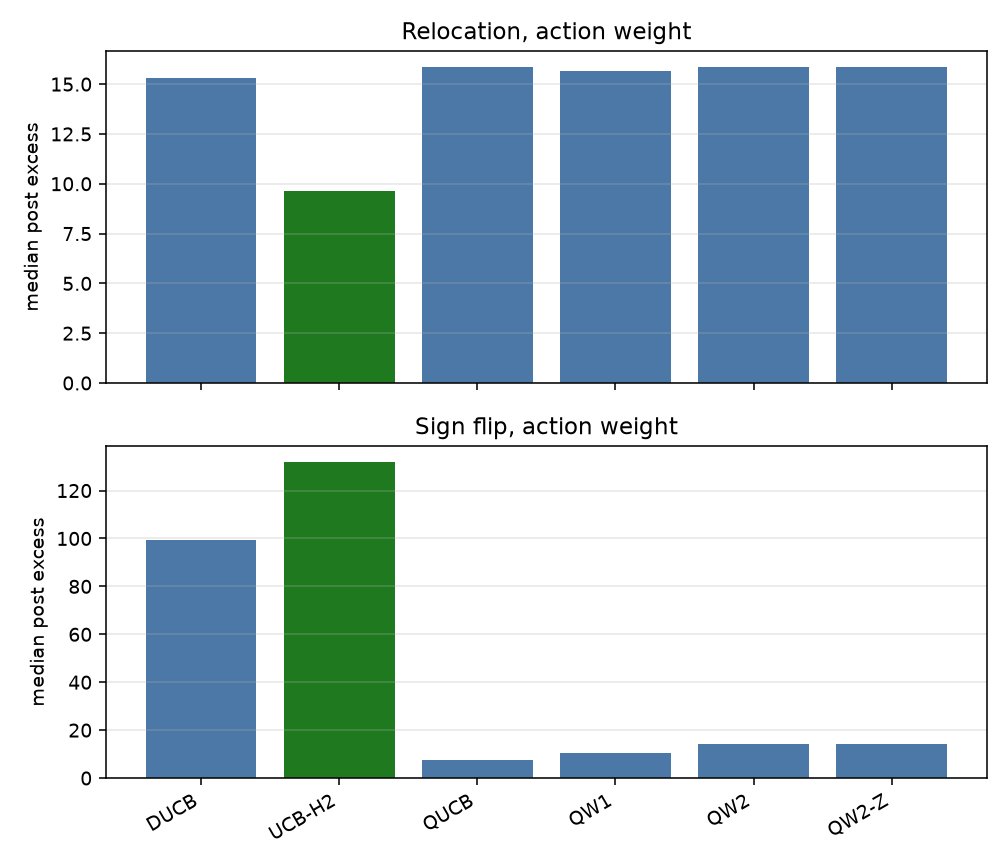
\includegraphics[width=0.92\textwidth]{weight_bars.png}
\caption{Median post-shift excess. The menu at \(\eta=2\) is marked in green.
QW1 and QW2 put the share on the action index. QW2-Z turns that weight off
when the zero policy holds the share.}
\end{figure}
\end{document}
